\documentclass{report}
\usepackage{geometry} % Page layout
\usepackage{multicol,caption} % Multiple columns
\usepackage{fancyhdr}
\usepackage{titlesec} % Section formatting
\usepackage{setspace} % Setting line spacing
\usepackage[normalem]{ulem} % Underline
\usepackage[backend=biber,style=apa,citestyle=authoryear]{biblatex}

\renewcommand*{\nameyeardelim}{\addcomma\space}
\DeclareDelimFormat[parencite]{finalnamedelim}{\addspace\&\space}
\addbibresource{references.bib}

\newenvironment{minifig}
  {\noindent\minipage{\linewidth}}
  {\endminipage}

\geometry{landscape, margin=0.5in}
\setlength{\columnsep}{1cm}
\setlength{\columnseprule}{0.5pt}
\pagenumbering{gobble}

\pagestyle{fancy}
\lhead{Jayden Lefebvre}
\rhead{SAFS 3530H Trent University}
\setlength{\headheight}{36pt}

\titleformat{\section}{\normalfont\fontsize{12}{15}\bfseries}{\thesection}{1em}{}

\begin{document}

\begin{center}
  \LARGE
  Ethylene Exposure and Shoot Growth in Early Vegetation of \textit{Narcissus sp.}
\end{center}

\medskip

\begin{multicols}{3}

  \textbf{Abstract}\\
  The effect of different concentrations of ethylene (C\textsubscript{2}H\textsubscript{4}) gas on plant bulb phenology is investigated.
  Apples are used as a source of ethylene gas in a closed greenhouse system, and bulb shoot height is measured over a period of five weeks.
  Final leaf height is plotted against with ethylene concentration, and leaf growth and growth rate are compared between control and ethylene-treated groups.
  Results were largely inconclusive, indicating poor experimental design or the influence of outside factors.
  
  \textbf{Introduction}\\
  Ethylene is a plant growth regulator responsible for fruit ripening and cell senescence.
  It has been reported in literature that exposure to ethylene can negatively impact plant shoot elongation in bulbous plants \parencite{bulbous}, and even induces leaf abscission (i.e. death) after long periods of exposure \parencite{abscission}.
  Literature findings indicate that the mechanism underlying these phenomena relate to the inhibition of auxin synthesis or enhancing auxin destruction \parencite{senescence}.
  The purpose of this study is to investigate the effect of ethylene exposure on the growth and growth rate of early vegetation in \textit{Narcissus sp.} bulbs.
  It is predicted that, due to the effect on auxin metabolism, ethylene exposure will inhibit shoot elongation in the early stages of plant growth.
  It is thus hypothesized that greater ethylene exposure will negatively influence leaf height in plant bulb vegetation.

  \vfill\null
  \columnbreak
  
  \textbf{Methods}\\
  % Each apparatus will have 1: pot (with soil and bulb), apple (excluding the control), skewer, cover and 2-4 elastic bands. The set-up apparatus will be a closed system that will contain the ethylene given off by the apple. Each plant pot and bulb is under one cover acting as a mini-greenhouse.
  Twenty-four (24) bulbs of daffodil (\textit{Narcissus sp.}) were planted individually in pots with organic nutrient-rich soil.
  Each pot was covered with a plastic cover, and a washed organic apple was placed inside the cover.
  The covered pot acted as a closed system to contain the ethylene given off by the apple.
  Ethylene concentration was measured at day 7.
  Leaf height was measured from the soil to the tip of the longest leaf using calipers on a (bi-)weekly basis for five weeks.

  \textbf{Results}\\
  Below are two graphs: Figure 1 shows the \textit{final} (day 35) leaf height vs ethylene concentration at day 7, with linear regression and coefficient of determination; Figure 2 shows the average leaf height over time per ethylene treatment \textit{group} (\textbf{Control}, \textbf{High} ethylene, and \textbf{Low} ethylene), each with line of best fit.

  \begin{minifig}
    \medskip
    \centering
    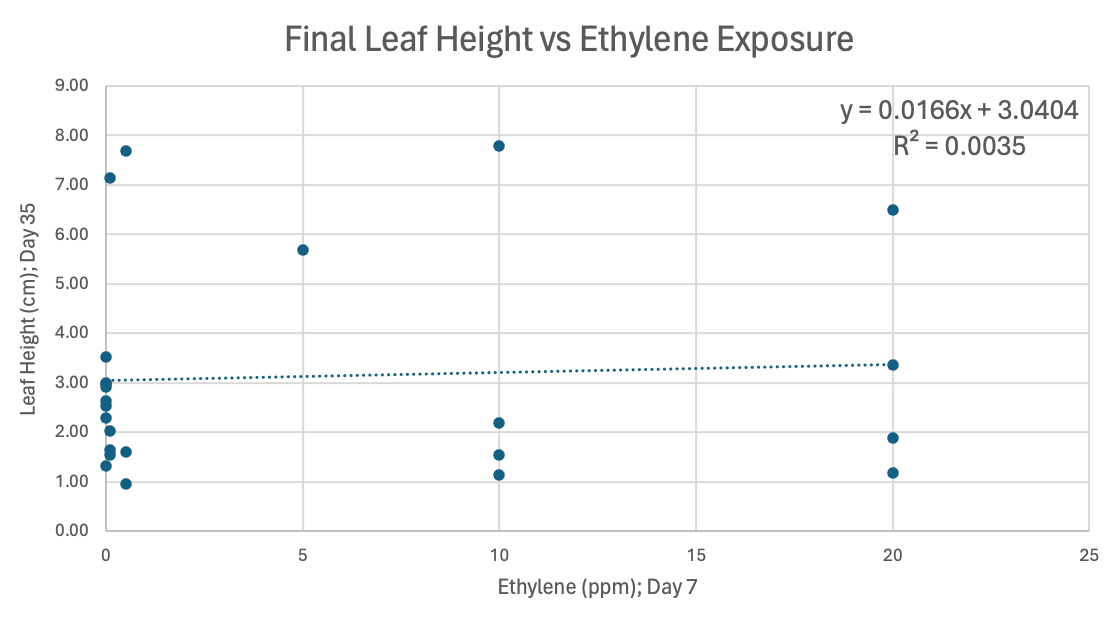
\includegraphics[width=\linewidth]{graph2.png}
    \captionof{figure}{Final (Day 35) leaf height vs ethylene concentration (Day 7) in \textit{Narcissus spp.} vegetation.}
    \medskip
  \end{minifig}
  \vfill\null
  \columnbreak
  \begin{minifig}
    \medskip
    \centering
    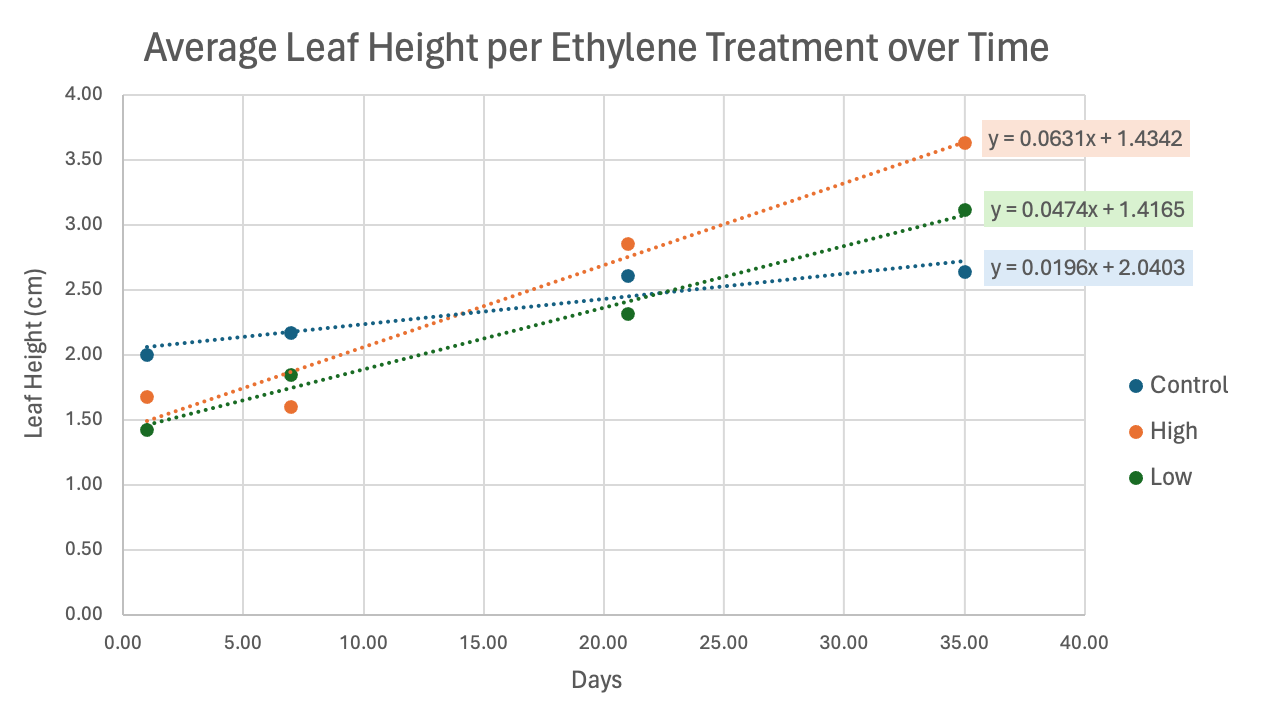
\includegraphics[width=\linewidth]{graph1.png}
    \captionof{figure}{Average leaf height per ethylene treatment in \textit{Narcissus spp.} vegetation over time.}
  \end{minifig}

  \textbf{Discussion}\\
  Increasing ethylene exposure did \uline{not} exhibit significant negative impact on final leaf height; \uline{no clear trend was observed} (R\textsuperscript{2} = 0.0035; Figure 1). In fact, the regression slope was slightly \textit{positive}, indicating a slight \textit{increase} in leaf height with increasing ethylene concentration. This is corroborated by data from Figure 2, which showed that ethylene-treated plants grew \textit{faster} and had a \textit{higher} final leaf height on average than control. ``In the presence of very low ethylene concentrations, [some plants] show increased leaf elongation rates'' \parencite{growth}; however, as low as 15ppm for as little as 72 hours has been shown to induce leaf abscission in ornamental plants \parencite{abscission}. Future research should focus on increasing the amount of ethylene data collected, i.e. frequency of measurement, experiment duration, and different concentrations. The results are \uline{inconclusive}, and the hypothesis is \uline{not supported}.
  
\end{multicols}

\clearpage

\setstretch{1.5}

\printbibliography

\end{document}